% Options for packages loaded elsewhere
% Options for packages loaded elsewhere
\PassOptionsToPackage{unicode}{hyperref}
\PassOptionsToPackage{hyphens}{url}
\PassOptionsToPackage{dvipsnames,svgnames,x11names}{xcolor}
%
\documentclass[
  authoryear,
  review,
  1p]{elsarticle}
\usepackage{xcolor}
\usepackage{amsmath,amssymb}
\setcounter{secnumdepth}{5}
\usepackage{iftex}
\ifPDFTeX
  \usepackage[T1]{fontenc}
  \usepackage[utf8]{inputenc}
  \usepackage{textcomp} % provide euro and other symbols
\else % if luatex or xetex
  \usepackage{unicode-math} % this also loads fontspec
  \defaultfontfeatures{Scale=MatchLowercase}
  \defaultfontfeatures[\rmfamily]{Ligatures=TeX,Scale=1}
\fi
\usepackage{lmodern}
\ifPDFTeX\else
  % xetex/luatex font selection
\fi
% Use upquote if available, for straight quotes in verbatim environments
\IfFileExists{upquote.sty}{\usepackage{upquote}}{}
\IfFileExists{microtype.sty}{% use microtype if available
  \usepackage[]{microtype}
  \UseMicrotypeSet[protrusion]{basicmath} % disable protrusion for tt fonts
}{}
\makeatletter
\@ifundefined{KOMAClassName}{% if non-KOMA class
  \IfFileExists{parskip.sty}{%
    \usepackage{parskip}
  }{% else
    \setlength{\parindent}{0pt}
    \setlength{\parskip}{6pt plus 2pt minus 1pt}}
}{% if KOMA class
  \KOMAoptions{parskip=half}}
\makeatother
% Make \paragraph and \subparagraph free-standing
\makeatletter
\ifx\paragraph\undefined\else
  \let\oldparagraph\paragraph
  \renewcommand{\paragraph}{
    \@ifstar
      \xxxParagraphStar
      \xxxParagraphNoStar
  }
  \newcommand{\xxxParagraphStar}[1]{\oldparagraph*{#1}\mbox{}}
  \newcommand{\xxxParagraphNoStar}[1]{\oldparagraph{#1}\mbox{}}
\fi
\ifx\subparagraph\undefined\else
  \let\oldsubparagraph\subparagraph
  \renewcommand{\subparagraph}{
    \@ifstar
      \xxxSubParagraphStar
      \xxxSubParagraphNoStar
  }
  \newcommand{\xxxSubParagraphStar}[1]{\oldsubparagraph*{#1}\mbox{}}
  \newcommand{\xxxSubParagraphNoStar}[1]{\oldsubparagraph{#1}\mbox{}}
\fi
\makeatother

\usepackage{color}
\usepackage{fancyvrb}
\newcommand{\VerbBar}{|}
\newcommand{\VERB}{\Verb[commandchars=\\\{\}]}
\DefineVerbatimEnvironment{Highlighting}{Verbatim}{commandchars=\\\{\}}
% Add ',fontsize=\small' for more characters per line
\usepackage{framed}
\definecolor{shadecolor}{RGB}{241,243,245}
\newenvironment{Shaded}{\begin{snugshade}}{\end{snugshade}}
\newcommand{\AlertTok}[1]{\textcolor[rgb]{0.68,0.00,0.00}{#1}}
\newcommand{\AnnotationTok}[1]{\textcolor[rgb]{0.37,0.37,0.37}{#1}}
\newcommand{\AttributeTok}[1]{\textcolor[rgb]{0.40,0.45,0.13}{#1}}
\newcommand{\BaseNTok}[1]{\textcolor[rgb]{0.68,0.00,0.00}{#1}}
\newcommand{\BuiltInTok}[1]{\textcolor[rgb]{0.00,0.23,0.31}{#1}}
\newcommand{\CharTok}[1]{\textcolor[rgb]{0.13,0.47,0.30}{#1}}
\newcommand{\CommentTok}[1]{\textcolor[rgb]{0.37,0.37,0.37}{#1}}
\newcommand{\CommentVarTok}[1]{\textcolor[rgb]{0.37,0.37,0.37}{\textit{#1}}}
\newcommand{\ConstantTok}[1]{\textcolor[rgb]{0.56,0.35,0.01}{#1}}
\newcommand{\ControlFlowTok}[1]{\textcolor[rgb]{0.00,0.23,0.31}{\textbf{#1}}}
\newcommand{\DataTypeTok}[1]{\textcolor[rgb]{0.68,0.00,0.00}{#1}}
\newcommand{\DecValTok}[1]{\textcolor[rgb]{0.68,0.00,0.00}{#1}}
\newcommand{\DocumentationTok}[1]{\textcolor[rgb]{0.37,0.37,0.37}{\textit{#1}}}
\newcommand{\ErrorTok}[1]{\textcolor[rgb]{0.68,0.00,0.00}{#1}}
\newcommand{\ExtensionTok}[1]{\textcolor[rgb]{0.00,0.23,0.31}{#1}}
\newcommand{\FloatTok}[1]{\textcolor[rgb]{0.68,0.00,0.00}{#1}}
\newcommand{\FunctionTok}[1]{\textcolor[rgb]{0.28,0.35,0.67}{#1}}
\newcommand{\ImportTok}[1]{\textcolor[rgb]{0.00,0.46,0.62}{#1}}
\newcommand{\InformationTok}[1]{\textcolor[rgb]{0.37,0.37,0.37}{#1}}
\newcommand{\KeywordTok}[1]{\textcolor[rgb]{0.00,0.23,0.31}{\textbf{#1}}}
\newcommand{\NormalTok}[1]{\textcolor[rgb]{0.00,0.23,0.31}{#1}}
\newcommand{\OperatorTok}[1]{\textcolor[rgb]{0.37,0.37,0.37}{#1}}
\newcommand{\OtherTok}[1]{\textcolor[rgb]{0.00,0.23,0.31}{#1}}
\newcommand{\PreprocessorTok}[1]{\textcolor[rgb]{0.68,0.00,0.00}{#1}}
\newcommand{\RegionMarkerTok}[1]{\textcolor[rgb]{0.00,0.23,0.31}{#1}}
\newcommand{\SpecialCharTok}[1]{\textcolor[rgb]{0.37,0.37,0.37}{#1}}
\newcommand{\SpecialStringTok}[1]{\textcolor[rgb]{0.13,0.47,0.30}{#1}}
\newcommand{\StringTok}[1]{\textcolor[rgb]{0.13,0.47,0.30}{#1}}
\newcommand{\VariableTok}[1]{\textcolor[rgb]{0.07,0.07,0.07}{#1}}
\newcommand{\VerbatimStringTok}[1]{\textcolor[rgb]{0.13,0.47,0.30}{#1}}
\newcommand{\WarningTok}[1]{\textcolor[rgb]{0.37,0.37,0.37}{\textit{#1}}}

\usepackage{longtable,booktabs,array}
\usepackage{calc} % for calculating minipage widths
% Correct order of tables after \paragraph or \subparagraph
\usepackage{etoolbox}
\makeatletter
\patchcmd\longtable{\par}{\if@noskipsec\mbox{}\fi\par}{}{}
\makeatother
% Allow footnotes in longtable head/foot
\IfFileExists{footnotehyper.sty}{\usepackage{footnotehyper}}{\usepackage{footnote}}
\makesavenoteenv{longtable}
\usepackage{graphicx}
\makeatletter
\newsavebox\pandoc@box
\newcommand*\pandocbounded[1]{% scales image to fit in text height/width
  \sbox\pandoc@box{#1}%
  \Gscale@div\@tempa{\textheight}{\dimexpr\ht\pandoc@box+\dp\pandoc@box\relax}%
  \Gscale@div\@tempb{\linewidth}{\wd\pandoc@box}%
  \ifdim\@tempb\p@<\@tempa\p@\let\@tempa\@tempb\fi% select the smaller of both
  \ifdim\@tempa\p@<\p@\scalebox{\@tempa}{\usebox\pandoc@box}%
  \else\usebox{\pandoc@box}%
  \fi%
}
% Set default figure placement to htbp
\def\fps@figure{htbp}
\makeatother





\setlength{\emergencystretch}{3em} % prevent overfull lines

\providecommand{\tightlist}{%
  \setlength{\itemsep}{0pt}\setlength{\parskip}{0pt}}



 
\usepackage[]{natbib}
\bibliographystyle{elsarticle-harv}


\makeatletter
\@ifpackageloaded{caption}{}{\usepackage{caption}}
\AtBeginDocument{%
\ifdefined\contentsname
  \renewcommand*\contentsname{Table of contents}
\else
  \newcommand\contentsname{Table of contents}
\fi
\ifdefined\listfigurename
  \renewcommand*\listfigurename{List of Figures}
\else
  \newcommand\listfigurename{List of Figures}
\fi
\ifdefined\listtablename
  \renewcommand*\listtablename{List of Tables}
\else
  \newcommand\listtablename{List of Tables}
\fi
\ifdefined\figurename
  \renewcommand*\figurename{Figure}
\else
  \newcommand\figurename{Figure}
\fi
\ifdefined\tablename
  \renewcommand*\tablename{Table}
\else
  \newcommand\tablename{Table}
\fi
}
\@ifpackageloaded{float}{}{\usepackage{float}}
\floatstyle{ruled}
\@ifundefined{c@chapter}{\newfloat{codelisting}{h}{lop}}{\newfloat{codelisting}{h}{lop}[chapter]}
\floatname{codelisting}{Listing}
\newcommand*\listoflistings{\listof{codelisting}{List of Listings}}
\makeatother
\makeatletter
\makeatother
\makeatletter
\@ifpackageloaded{caption}{}{\usepackage{caption}}
\@ifpackageloaded{subcaption}{}{\usepackage{subcaption}}
\makeatother
\journal{Journal of Transport Geography}
\usepackage{bookmark}
\IfFileExists{xurl.sty}{\usepackage{xurl}}{} % add URL line breaks if available
\urlstyle{same}
\hypersetup{
  pdftitle={Multidimensional Transport Poverty Index},
  pdfauthor={Miguel Alvelos; Mauricio Orozco-Fontalvo; Gonçalo F. Matos; Rosa Félix; Camila Garcia; Filipe Moura},
  pdfkeywords={keyword1, keyword2},
  colorlinks=true,
  linkcolor={blue},
  filecolor={Maroon},
  citecolor={Blue},
  urlcolor={Blue},
  pdfcreator={LaTeX via pandoc}}


\setlength{\parindent}{6pt}
\begin{document}

\begin{frontmatter}
\title{Multidimensional Transport Poverty Index \\\large{A replicable
multi-dimensional and multi-modal measure of transport poverty} }
\author[1]{Miguel Alvelos%
\corref{cor1}%
}
 \ead{miguel.alvelos@tecnico.ulisboa.pt} 
\author[1]{Mauricio Orozco-Fontalvo%
%
}
 \ead{mauricio.orozco@tecnico.ulisboa.pt} 
\author[1]{Gonçalo F. Matos%
%
}
 \ead{goncaloafmatos@tecnico.ulisboa.pt} 
\author[1]{Rosa Félix%
%
}
 \ead{rosamfelix@tecnico.ulisboa.pt} 
\author[2]{Camila Garcia%
%
}
 \ead{camila.garcia@tmlmobilidade.pt} 
\author[]{Filipe Moura%
%
}
 \ead{fmoura@tecnico.ulisboa.pt} 

\affiliation[1]{organization={CERIS, Instituto Superior Técnico -
Universidade de Lisboa},addressline={Av Rovisco Pais 1},city={1049-001
Lisbon},postcode={Portugal},postcodesep={}}
\affiliation[2]{organization={Transportes Metropolitanos de
Lisboa},addressline={Rua da Cruz de Santa Apolónia 23},city={1100-187
Lisbon},postcode={Portugal},postcodesep={}}

\cortext[cor1]{Corresponding author}






        
\begin{abstract}
This is the abstract. Lorem ipsum dolor sit amet, consectetur adipiscing
elit. Vestibulum augue turpis, dictum non malesuada a, volutpat eget
velit. Nam placerat turpis purus, eu tristique ex tincidunt et. Mauris
sed augue eget turpis ultrices tincidunt. Sed et mi in leo porta
egestas. Aliquam non laoreet velit. Nunc quis ex vitae eros aliquet
auctor nec ac libero. Duis laoreet sapien eu mi luctus, in bibendum leo
molestie. Sed hendrerit diam diam, ac dapibus nisl volutpat vitae.
Aliquam bibendum varius libero, eu efficitur justo rutrum at. Sed at
tempus elit.
\end{abstract}





\begin{keyword}
    keyword1 \sep 
    keyword2
\end{keyword}
\end{frontmatter}
    

\section{Introduction}\label{sec-introduction}

Transportation is an essential service which can condition access to
almost all human activities, be them work, education, health or social
life. When this access is limited by insufficient supply, high costs, or
elevated exposure to systemic risks and externalities, the term
Transport Poverty is used \citep{Lucas_2016}. This phenomenon has direct
consequences in social exclusion and territorial cohesion
\citep{MejiaDorantes_MurauskaiteBull_2022}.

In the European context, this problem has increased its political
relevance over the last decade. The European Pillar of Social Rights, in
its 20th Principle, enshrines the right to access essential services,
including transportation. Regulation (EU) 2023/955 of 10 May 2023, which
established the Social Climate Fund (SCF), enshrined the first legally
bounding definition of transport poverty at an European scale, defining
it as ``individuals' and households' inability or difficulty to meet the
costs of private or public transport, or their lack of or limited access
to transport needed for their access to essential socioeconomic services
and activities, taking into account the national and spatial context''
\citep{EU_2023955} .

Despite the clear empirical relevance of this phenomenon, there is
difficulty in quantifying it in a systematic way. Specifically in
Portugal, previous research has focused on punctual case studies
\citep{Pritchard_2014} or on costly mobility surveys
\citep{INE_IMOB2017}, which can hardly be renewed at the cadence
required by public policy cycles.

This project was thus developed in an attempt to bridge the existing
methodological gap with the creation of a composite and intermodal tool
- the Multidimensional Transport Poverty Index (IMPT) - that is
replicable and scalable, as well as wholly based in public data,
intended to assist and support public policy instruments, such as the
European Union's Social Climate Fund (SCF) or Sustainable Urban Mobility
Plans (SUMPs). The Lisbon Metropolitan Area (LMA) was employed as a case
study for the tool's validation.

\section{Literature review}\label{sec-literature_review}

\subsection{Definitions of Transport Poverty}\label{sec-LR_definitions}

Transport systems are a fundamental part of modern society, and their
absence is related to social exclusion - a state where an individual or
a societal group is left out of participating in regular social
activities in a given society \citep{Pritchard_2014} -,
socio-territorial inequality and transport inequality - the differences
in transport conditions for different groups of people
\citep{Hidayati_2021}. Despite the relation between poverty and
transport conditions, these are also related to a wide range of social
issues, with motorized vehicle users most contributing to externalities,
but with vulnerable road users being disproportionately affected by them
in health, space allocation and time consumption \citep{Gossling_2016}.
Moreover, lower-income households tend to not have financial conditions
to have motorized transport or to reside in central areas, relegating
them to live in areas distant from the city center, often poorly served
by public transportation. \citep{Fedorowicz_2020} \citep{Lopes_2023}.

These differences in transport conditions can lead to transport poverty,
a concept which lacks a single universally accepted definition in
scientific literature. This expression has been used to broadly describe
inequities related with transportation access, but also in a more
restricted way to refer to the economic inability to support
transportation costs \citep{Mattioli_2018}. However, as
\citet{Lucas_2016} states, different terminologies relating to transport
poverty - terms such as ``mobility poverty'', ``accessibility poverty''
or ``transport disadvantage'' - are used with ``often very different,
although also overlapping definitions''. Due to this lack of a universal
definition and the multidimensional nature of transport poverty, its
measurement and quantification poses a challenge
\citep{Levinson_King_2020}.

This way, the necessity to comprehend this concept and quantify it
becomes more urgent. It is essential to define reliable indicators of
transport vulnerability to map ``public transport deserts''
\citep{Jiao_Dillivan_2013} and low-accessibility areas in order to
inform public intervention and to monitor the implementation of measures
to improve these situations. A reliable and replicable index to measure
transport poverty is thus fundamental to support public policy
instruments.

\citet{Lucas_2016} proposes the most comprehensive conceptual
systematization of transport poverty, clearly defining previously
different but overlapping terminology. They define transport poverty as
a combination of the following four dimensions:

\begin{itemize}
\tightlist
\item
  Accessibility - the capacity to reach usual destinations and
  activities (work, education, health and so on).
\item
  Mobility - the systemic lack of transportation that impacts trips.
\item
  Affordability - the ability to meet the cost of transportation.
\item
  Exposure to externalities (Safety) - the negative exposure to the
  transport system itself, such as disproportional rates of pollution or
  road crashes.
\end{itemize}

Recently, and based on the aforementioned concepts,
\citet{MejiaDorantes_MurauskaiteBull_2022} have proposed a definition
that has been widely adopted: transport poverty is the inability of an
individual or household to access essential services or opportunities
due to transportation services that are inaccessible, inadequate,
unaffordable, time-consuming or unsafe. This definition has been adapted
and applied at the European scale, through \citet{EU_2023955} and a
recent European Commission Report \citep{EuropeanCommission_2024}. The
key dimensions in the EC Report are synthesized as \emph{Availability}
(corresponding to Lucas' Mobility), \emph{Accessibility} and
\emph{Affordability}, with exposure to externalities being included in
the overarching concept of \emph{Adequacy}.

In summary, the concept of transport poverty has evolved from a
one-dimensional look at accessibility or affordability, to a composite
approach that attempts to capture the multidimensional nature of this
phenomenon.

During the last decade various interactive spatial tools based on
indicators of accessibility and inequality have been created and made
publicly available. Two of these are here highlighted, due to their
conceptual or methodological influence and their proximity to the IMPT's
objective.

\subsection{Dimensions of Transport Poverty}\label{sec-LR_dimensions}

The dimensions proposed by \citet{Lucas_2016} continue to be the
reference for composite indexes of transport poverty
\citep{AlonsoEpelde_2023} \citep{MejiaDorantes_MurauskaiteBull_2022}.
IMPT adopts these dimensions, implementing them through secondary data
available in Portugal. Each of them is further explained thoroughly.

\subsubsection{Accessibility}\label{sec-LR_accessibility}

Accessibility refers to the ability to reach regular destinations such
as employment, education, health and other essential services
\citep{Allen_Farber_2019} \citep{SocialExclusionUnit_2003}.

\subsubsection{Mobility}\label{sec-LR_mobility}

Mobility refers to the systemic deficits of the transport system, be
them lack of infrastructure, lack of service frequency or long trip
duration \citep{Levinson_King_2020} \citep{Lucas_2016}
\citep{MejiaDorantes_MurauskaiteBull_2022}. This dimension captures
different aspects of transport supply that accessibility is not able to,
their core difference being that, while accessibility asks which places
are reachable, mobility focuses on how easy it is to reach them.

\subsubsection{Affordability}\label{sec-LR_affordability}

\subsubsection{Safety}\label{sec-LR_safety}

This dimension is commonly not included in transport poverty indexes
\citep{Kelly_2023}, being considered only in the most wide-ranging
definitions of transport poverty \citep{Lucas_2016}
\citep{UNHabitat_2013}. It refers to the exposure to externalities of
the transport system, such as road crashes and pollution, which have
disproportionate effects on the territory. For the IMPT, this
dimension's inputs only included those related to road safety
indicators, due to the inability to get open and granular data regarding
environmental externalities.

A fifth dimension, digital literacy, was initially considered as a proxy
for access to information and mobility services \citep{Durand_2022}
\citep{OrozcoFontalvo_2025} \citep{Velaga_2012}. However, it was
excluded from the final implementation of the index due to
unavailability of data compatible with the scale of the lowest
administrative division.

\subsection{IMPT's Contribution}\label{sec-LR_contribution}

IMPT emerges in an attempt to create an index synthesizing these
dimensions and providing a reliable measurement of transport poverty,
bridging three gaps in the literature and in national public policy.

\begin{enumerate}
\def\labelenumi{\arabic{enumi}.}
\tightlist
\item
  There is, in Portugal, the absence of an index that integrates the
  four aforementioned dimensions across multiple transport modes and is
  replicable at the lowest administrative level.
\item
  Existing indexes excessively depend on costly primary data that is
  difficult to monitor continuously. IMPT relies exclusively on
  secondary and open data, easily allowing for updates and monitoring
  over time.
\item
  There is a lack of operational tools that allow to translate academic
  literature on transport poverty into decision-support instruments for
  local governments, transport authorities, and generally public policy
  makers.
\end{enumerate}

Furthermore, the IMPT incorporates four methodological variants,
corresponding to different analytical positions:

\begin{itemize}
\tightlist
\item
  Contrasting IMPT: based on entropy, highlights the variables with the
  highest variation, better capturing territorial contrasts.
\item
  Critical IMPT: based on the geometric mean, it non-linearly penalizes
  the dimensions with the worst performance in each area.
\item
  Balanced IMPT: based on the arithmetic mean, allows for compensation
  between dimensions.
\item
  Political IMPT: allowing for a personalized AHP weighting, it can be
  tailored to the decision-maker's preferences.
\end{itemize}

If \texttt{cite-method} is set to \texttt{citeproc} in
\texttt{elsevier\_article()}, then pandoc is used for citations instead
of \texttt{natbib}. In this case, the \texttt{csl} option is used to
format the references. By default, this template will provide an
appropriate style, but alternative \texttt{csl} files are available from
\url{https://www.zotero.org/styles?q=elsevier}. These can be downloaded
and stored locally, or the url can be used as in the example header.

Here are two sample references: \citet{Pereira_r5r_2021}
\citet{INE_IMOB2017}. If citing the other way \citep{Lovelace_2022}.

\section{Methodology}\label{sec-methodology}

\subsection{Case Study}\label{sec-MET_case_study}

The Lisbon Metropolitan Area (LMA) was applied as the case study for the
IMPT. The LMA is comprised of two NUTS II regions (Grande Lisboa and
Península de Setúbal), which encompasses 18 Municipalities and
approximately 2,8 million inhabitants. This region presents territorial
characteristics which make it particularly suitable for this analysis: a
polycentric structure with a strong employment center in Lisbon,
significant discrepancies between the public transport offer in the
urban core and in the periphery, and a high modal share of private
vehicles in a large part of the metropolitan area.

The analysis is focused on the lowest administrative division, the
\emph{freguesia} (parish), which is the most disaggregated geographical
level that guarantees data coverage for all utilized sources. For the
indicators that had a higher level of granularity, an analysis by grid
level was also assembled. The LMA includes 124 parishes, which
constitute the observation units of the IMPT.

\subsubsection{Data Sources}\label{sec-MET_data_sources}

Lastly, the following R packages were utilized in the data processing
and creation of both the index and its interactive dashboard:
\texttt{readr,\ readxl,\ openxlsx,\ lubridate,\ dplyr,\ tidyr,\ stringr,\ tidyverse,\ sf,\ terra,\ mapview,\ stplanr,\ h3jsr,\ r5r,\ accessibility,\ odjitter,\ tidytransit,\ GTFShift,\ FactoMineR,\ assertthat,\ piggyback}.

\subsection{Each Dimension's Indicators}\label{sec-MET_indicators}

The IMPT is not only multidimensional, but also intermodal. In
Table~\ref{tbl-modes_per_dimension}, the dimensions used to compute the
index for each mode are specified.

\begin{Shaded}
\begin{Highlighting}[]
\NormalTok{modes\_per\_dimension }\OtherTok{\textless{}{-}} \FunctionTok{data.frame}\NormalTok{(}
  \AttributeTok{Dimension =} \FunctionTok{c}\NormalTok{(}\StringTok{"Accessibility"}\NormalTok{,}
                \StringTok{"Mobility"}\NormalTok{,}
                \StringTok{"Affordability"}\NormalTok{,}
                \StringTok{"Safety"}
\NormalTok{                ),}
  \AttributeTok{Mode =} \FunctionTok{c}\NormalTok{(}\StringTok{"Driving, Public Transport, Walking, Cycling"}\NormalTok{,}
           \StringTok{"Driving, Public Transport, Walking, Cycling"}\NormalTok{,}
           \StringTok{"Driving, Public Transport"}\NormalTok{,}
           \StringTok{"Driving, Walking, Cycling"}
\NormalTok{           )}
\NormalTok{)}
\NormalTok{knitr}\SpecialCharTok{::}\FunctionTok{kable}\NormalTok{(modes\_per\_dimension)}
\end{Highlighting}
\end{Shaded}

\begin{verbatim}
Warning in attr(x, "align"): 'xfun::attr()' is deprecated.
Use 'xfun::attr2()' instead.
See help("Deprecated")
\end{verbatim}

\begin{verbatim}
Warning in attr(x, "format"): 'xfun::attr()' is deprecated.
Use 'xfun::attr2()' instead.
See help("Deprecated")
\end{verbatim}

\begin{longtable}[]{@{}ll@{}}

\caption{\label{tbl-modes_per_dimension}Modes evaluated in each
dimension}

\tabularnewline

\toprule\noalign{}
Dimension & Mode \\
\midrule\noalign{}
\endhead
\bottomrule\noalign{}
\endlastfoot
Accessibility & Driving, Public Transport, Walking, Cycling \\
Mobility & Driving, Public Transport, Walking, Cycling \\
Affordability & Driving, Public Transport \\
Safety & Driving, Walking, Cycling \\

\end{longtable}

\subsubsection{Accessibility}\label{sec-MET_accessibility}

The Accessibility dimension quantifies the capacity to reach key
destinations within a given travel time threshold. The key destination
categories, as well as their data sources, are summarized in table
(\ldots)

This dimension incorporates two metrics:

\begin{enumerate}
\def\labelenumi{\arabic{enumi}.}
\tightlist
\item
  Cumulative number of opportunities: number of points of interest of a
  given category reachable within a certain amount of time.
\item
  Travel time to reach nearest opportunities: time required to reach the
  first \emph{n} opportunities of a given category.
\end{enumerate}

Indicators for this dimension were computed using the H3 grid
\citep{Uber_H3_2018} of resolution 8 \citep{Pereira_accessibility_2022},
which corresponds to 3686 hexagons in the LMA, with an edge length of
531 meters and an average hexagon area of approximately 737,327m².

\paragraph{Jittering}\label{sec-MET_jittering}

Due to a lack of open access to fine data regarding job location, the
most granular data obtained was an OD matrix at the parish level,
provided by \citet{INE_IMOB2017}, with centroid to centroid
representations, ``a common approach involving the simplifying
assumption that all trip destinations and origins can be represented by
(sometimes population weighted or aggregated) zone centroids''
\citep{Lovelace_2022}. However, in order to accurately compute
accessibility and mobility measures, there was the need to have more
disaggregated data regarding job locations, beyond the parish unit.

This way, jittering \citep{Lovelace_2022} was used as a proxy for this
purpose, using building volumes as trip attractors, and this way
weighting origins and destinations. This allowed for the disaggregation
of trips between parishes to ODs with up to 50 trips.

\paragraph{Travel time matrix}\label{sec-MET_TTmatrix}

A travel time matrix was used as the basis for all accessibility
measures. It was computed between each grid cell, over a network
\citep{Pereira_r5r_2021} that was built considering:

\begin{itemize}
\item
  OpenStreetMap road network, exported from \citet{hot_osm}.
\item
  General Transit Feed Specification (GTFS) for all operators in the LMA
  (valid at 04/02/2026).
\item
  Terrain elevation profile \citep{copernicus_browser}.
\end{itemize}

The matrix was computed using the function
\texttt{r5r::travel\_time\_matrix()} with the following parameters: ()

\paragraph{Cumulative number of
opportunities}\label{sec-MET_Nopportunities}

The cumulative number of opportunities was calculated using the function
\texttt{accessibility::cumulative\_cutoff()} considering the travel time
matrices for each grid cell combination, the number of opportunities per
grid cell, and the travel time cut-offs.

This measure was computed for all combinations of POIs and modes for
time cut-offs of 5, 10, 15, 30, 45, 60, 75 and 90 minutes. However, as
can be seen in Table~\ref{tbl-accessibility_n_opportunities}, only
selected combinations of modes/points of interest were included in
IMPT's operationalization.

\begin{Shaded}
\begin{Highlighting}[]
\NormalTok{accessibility\_n\_opportunities }\OtherTok{\textless{}{-}} \FunctionTok{data.frame}\NormalTok{(}
  \StringTok{"Point of Interest/Mode"} \OtherTok{=} \FunctionTok{c}\NormalTok{(}\StringTok{"Healthcare Facilities"}\NormalTok{,}
                               \StringTok{"Basic Education"}\NormalTok{,}
                               \StringTok{"Green Spaces"}\NormalTok{,}
                               \StringTok{"Recreation"}\NormalTok{,}
                               \StringTok{"Groceries"}\NormalTok{,}
                               \StringTok{"Jobs"}
\NormalTok{                               ),}
  \StringTok{"Driving or Public Transport"} \OtherTok{=} \FunctionTok{c}\NormalTok{(}\StringTok{"30"}\NormalTok{,}\StringTok{"30"}\NormalTok{,}\StringTok{"5{-}10"}\NormalTok{,}\StringTok{"5{-}10"}\NormalTok{,}\StringTok{"15"}\NormalTok{,}\StringTok{"30{-}45"}\NormalTok{),}
  \StringTok{"Walking or Cycling"} \OtherTok{=} \FunctionTok{c}\NormalTok{(}\StringTok{"15"}\NormalTok{,}\StringTok{"15"}\NormalTok{,}\StringTok{"15{-}30"}\NormalTok{,}\StringTok{"15{-}30"}\NormalTok{,}\StringTok{"15"}\NormalTok{,}\StringTok{"30{-}45"}\NormalTok{),}
  \AttributeTok{check.names =} \ConstantTok{FALSE}
\NormalTok{)}
\NormalTok{knitr}\SpecialCharTok{::}\FunctionTok{kable}\NormalTok{(accessibility\_n\_opportunities)}
\end{Highlighting}
\end{Shaded}

\begin{verbatim}
Warning in attr(x, "align"): 'xfun::attr()' is deprecated.
Use 'xfun::attr2()' instead.
See help("Deprecated")
\end{verbatim}

\begin{verbatim}
Warning in attr(x, "format"): 'xfun::attr()' is deprecated.
Use 'xfun::attr2()' instead.
See help("Deprecated")
\end{verbatim}

\begin{longtable}[]{@{}
  >{\raggedright\arraybackslash}p{(\linewidth - 4\tabcolsep) * \real{0.3286}}
  >{\raggedright\arraybackslash}p{(\linewidth - 4\tabcolsep) * \real{0.4000}}
  >{\raggedright\arraybackslash}p{(\linewidth - 4\tabcolsep) * \real{0.2714}}@{}}

\caption{\label{tbl-accessibility_n_opportunities}Travel time threshold
(minutes) to compute cumulative number of opportunities}

\tabularnewline

\toprule\noalign{}
\begin{minipage}[b]{\linewidth}\raggedright
Point of Interest/Mode
\end{minipage} & \begin{minipage}[b]{\linewidth}\raggedright
Driving or Public Transport
\end{minipage} & \begin{minipage}[b]{\linewidth}\raggedright
Walking or Cycling
\end{minipage} \\
\midrule\noalign{}
\endhead
\bottomrule\noalign{}
\endlastfoot
Healthcare Facilities & 30 & 15 \\
Basic Education & 30 & 15 \\
Green Spaces & 5-10 & 15-30 \\
Recreation & 5-10 & 15-30 \\
Groceries & 15 & 15 \\
Jobs & 30-45 & 30-45 \\

\end{longtable}

The value computed represents the number of opportunities reachable
within the defined travel time threshold. Values at parish and
municipality level are aggregated considering a weighted mean of the
number of opportunities reachable in each grid cell within that
geographical unit, weighted by the population of those cells.

\paragraph{Travel time to reach closest
opportunities}\label{sec-MET_TTopportunities}

This measure was computed using the function
\texttt{accessibility::cost\_to\_closest()}, considering the travel time
matrices for each grid cell combination and the number of opportunities
in each grid cell. Its output corresponds to the travel cost, in
minutes, to reach \emph{n} opportunities of a certain category. Although
calculations were performed for 1, 2 and 3 opportunities, only some of
these were included in IMPT's operationalization, depending on the POI
category:

\begin{itemize}
\item
  Healthcare, basic education and green spaces: 1 opportunity.
\item
  Recreation, groceries and jobs: 3 opportunities.
\end{itemize}

\subsubsection{Mobility}\label{sec-MET_mobility}

Mobility evaluates the quality of the transportation system as a
service, independently of the accessibility of the destinations. The
methodology to calculate its principal indicators is explained and
detailed below.

\paragraph{Average commuting time}\label{average-commuting-time}

Using the jittered OD pairs from \citet{INE_IMOB2017} (for commuting)
and the travel time matrices, average commuting travel times are
computed for each geographical unit and mode, weighted by number of
trips. Trips with no feasible route within the constraints are assigned
the maximum travel time (120 min) and counted separately as ``not
accomplishable'' trips (PNA - Percentagem Não Alcançáveis).

\paragraph{Average number of commuting
transfers}\label{average-number-of-commuting-transfers}

For each commuting OD pair, the minimum number of transfers required for
each public transport route (for 0, 1, 2, and 3 transfers) is assigned
to each OD pair, and population-weighted mean transfers are computed per
geographical unit. The result is the average minimum amount of transfers
to commute to work using public transport.

\paragraph{Public transport headways and waiting
times}\label{public-transport-headways-and-waiting-times}

\paragraph{Public transport population
coverage}\label{public-transport-population-coverage}

\paragraph{Ratio of pedestrian and cycling
infrastructure}\label{ratio-of-pedestrian-and-cycling-infrastructure}

\paragraph{Shared mobility
availability}\label{shared-mobility-availability}

\subsubsection{Affordability}\label{sec-MET_affordability}

Affordability evaluates the capacity of households to support the
monetary costs of transportation to access essential activities. IMPT
uses a weighted cost by mode, in which the monetary cost of
automobile/public transport travel is multiplied by each parish's modal
share, and expressed as a proportion of median household income. The
travel costs are estimated for one-way trips from home to the workplace
during the morning peak.

\paragraph{Cost of driving}\label{sec-MET_cost_driving}

\paragraph{Cost of public transportation}\label{sec-MET_cost_PT}

\paragraph{Composite measures}\label{sec-MET_aff_composite}

\subsubsection{Safety}\label{sec-MET_safety}

This dimension encompasses the disproportional exposure to externalities
of the transportation system. It is entirely based on road safety data
provided by Autoridade Nacional de Segurança Rodoviária (ASNR) through
Transportes Metropolitanos de Lisboa (TML) \citep{pmmus}. It is
important to note that only road crashes occuring \emph{inside
localities} (dentro das localidades), a category specified by the ASNR
itself, are included in the index. In particular, this excludes crashes
on motorways and on the two bridges crossing the Tagus river, while
maintaining IMPT's spatial scope.

The indicators calculated for each geographical unit and transport mode
are systematized below:

\begin{itemize}
\tightlist
\item
  Total accidents (5 years): \[\sum(Acc_{5y})\]
\item
  Fatalities (30-day): \[\sum(VM_{30d})\]
\item
  Serious injuries (30-day): \[\sum(FG_{30d})\]
\item
  Slight injuries (30-day): \[\sum(FL_{30d})\]
\item
  Accident rate: \[\frac{\sum(Acc_{5y})}{Population} \times 1000\]
\item
  Fatality rate: \[\frac{\sum(VM_{30d})}{Population} \times 1000\]
\item
  Severity index (total): \[\frac{\sum(VM_{30d})}{\sum(Acc_{5y})}\]
\item
  Severity index (motorized):
  \[\frac{\sum(VM_{30d})}{Motorized\; vehicles\; involved}\]
\item
  Severity index (cycling):
  \[\frac{\sum(VM_{30d})}{Cyclists\; involved}\]
\item
  Severity index (pedestrian):
  \[\frac{\sum(VM_{30d})}{Pedestrians\; involved}\]
\end{itemize}

\subsection{Normalization and
Aggregation}\label{sec-MET_normalisation_aggregation}

All indicators are normalized to the range {[}1, 100{]} using min-max
scaling:

\textbf{For benefit indicators} (higher raw value → better):
\[X_{norm} = 1 + \frac{X - X_{min}}{X_{max} - X_{min}} \times 99\]

\textbf{For cost indicators} (lower raw value → better):
\[X_{norm} = 1 + \frac{X_{max} - X}{X_{max} - X_{min}} \times 99\]

\begin{itemize}
\tightlist
\item
  \textbf{Accessibility} metrics (\texttt{access\_*}) are \emph{benefit}
  indicators.
\item
  \textbf{Mobility} cost metrics (\texttt{mobility\_cost\_*}), public
  transport waiting times, all \textbf{affordability} indicators, and
  all \textbf{safety} indicators are \emph{cost} indicators.
\end{itemize}

Missing values in accessibility indicators (arising from unfeasible
public transportation routes) are imputed with the mean of the
respective variable prior to PCA.

\subsection{PCA-Based Dimension Scores}\label{sec-MET_pca}

For each dimension (Accessibility, Mobility, Safety) and at the global
(all-mode) and per-mode levels, a PCA is run using
\texttt{FactoMineR::PCA()} at parish level.

The \textbf{first principal component (PC1)} score is used as the
dimension index, after rescaling to {[}1, 100{]}. PC1 captures the
dominant axis of variation among the normalised indicators.

For \textbf{Affordability}, PCA is not applied (too few indicators);
instead, the normalised composite \texttt{h\_transp\_inc\_comp} (housing
+ transport cost as share of income, modal-share weighted) is used
directly as the Affordability Index.

For \textbf{Safety per mode}, an equal-weight average of the severity
index (per mode) and total vehicles involved (per mode) is used instead
of PCA.

For \textbf{Mobility - Car} PCA is not applied (too few indicators);
instead, we assumed an equal-weight average of the normalized composite
\texttt{mobility\_commuting\_avg\_tt\_car} and \texttt{road\_length}.

\subsection{Composite IMPT Scores}\label{sec-MET_composite_impt}

Three aggregation methods are computed for the global IMPT and each
per-mode IMPT:

\begin{enumerate}
\def\labelenumi{\arabic{enumi}.}
\tightlist
\item
  \textbf{Geometric mean} (equal weights,
  Figure~\ref{fig-imt-geometric}):
  \[IMPT_{geom} = \left(\prod_{d} (S_d + 1)\right)^{1/n} - 1\]
\end{enumerate}

Partially compensatory: penalizes dimensions with very low values
non-linearly. Highlights the most critical situations, where at least
one dimension is severely deficient.

\begin{enumerate}
\def\labelenumi{\arabic{enumi}.}
\setcounter{enumi}{1}
\tightlist
\item
  \textbf{Arithmetic mean} (equal weights,
  Figure~\ref{fig-imt-arithmetic}):
  \[IMPT_{avg} = \frac{1}{n} \sum_d S_d\]
\end{enumerate}

Compensatory: high vulnerability in one dimension can be offset by good
performance in others. Suitable for setting aggregate policy targets and
communicating to non-specialist audiences.

\begin{enumerate}
\def\labelenumi{\arabic{enumi}.}
\setcounter{enumi}{2}
\tightlist
\item
  \textbf{Entropy-weighted geometric mean}
  (Figure~\ref{fig-imt-entropy}):
  \[IMPT_{entropy} = \prod_d (S_d + 1)^{w_d} - 1\]
\end{enumerate}

where weights \(w_d\) are derived from the \textbf{entropy weighting
method}:

Weights are determined by the empirical dispersion of the dimensions
across parishes: the dimension that varies most among territories
receives greater weight. Maximises territorial contrast and is useful
for competitive prioritisation of interventions.

\[w_d = \frac{d_d}{\sum_j d_j}, \quad d_d = 1 - e_d, \quad e_d = -k \sum_i p_{id} \ln(p_{id})\]

with \(k = 1/\ln(n)\) and \(p_{id}\) being the proportion of the
dimension score for area \(i\).

\begin{figure}

\begin{minipage}{0.33\linewidth}

\centering{

\pandocbounded{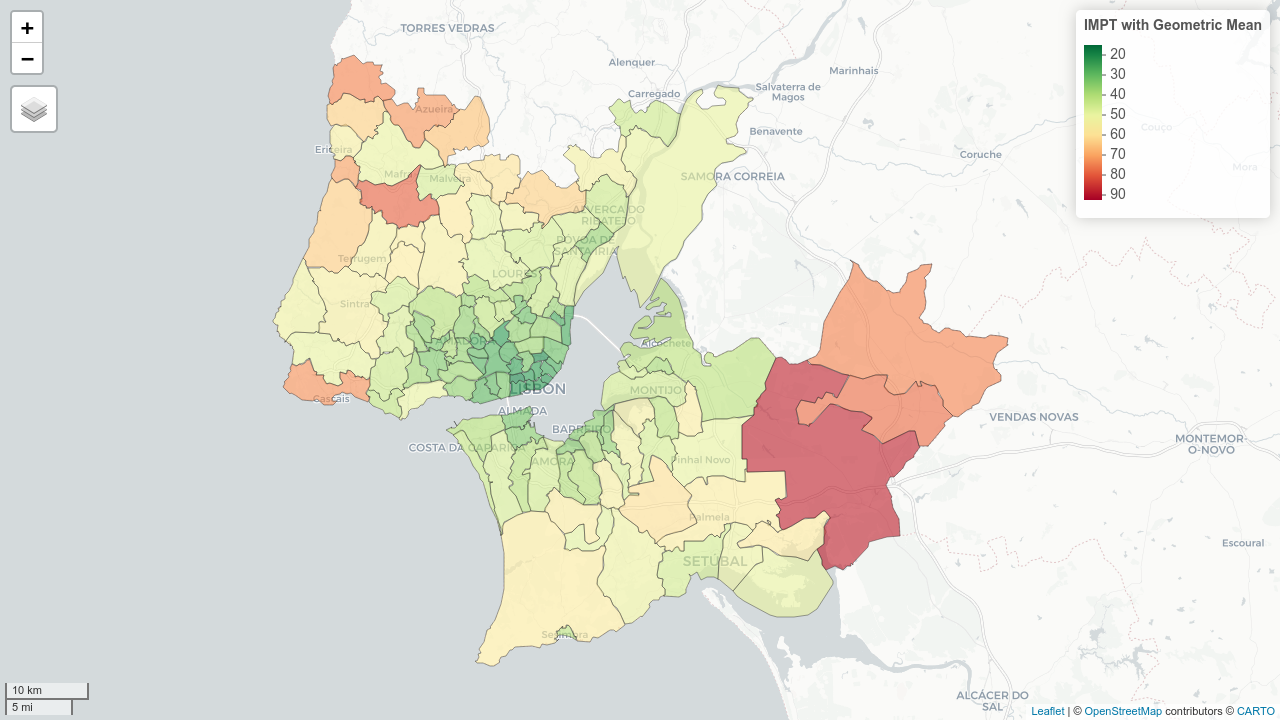
\includegraphics[keepaspectratio]{../documents/images/maps/impt_geometric.png}}

}

\subcaption{\label{fig-imt-geometric}Geometric mean}

\end{minipage}%
%
\begin{minipage}{0.33\linewidth}

\centering{

\pandocbounded{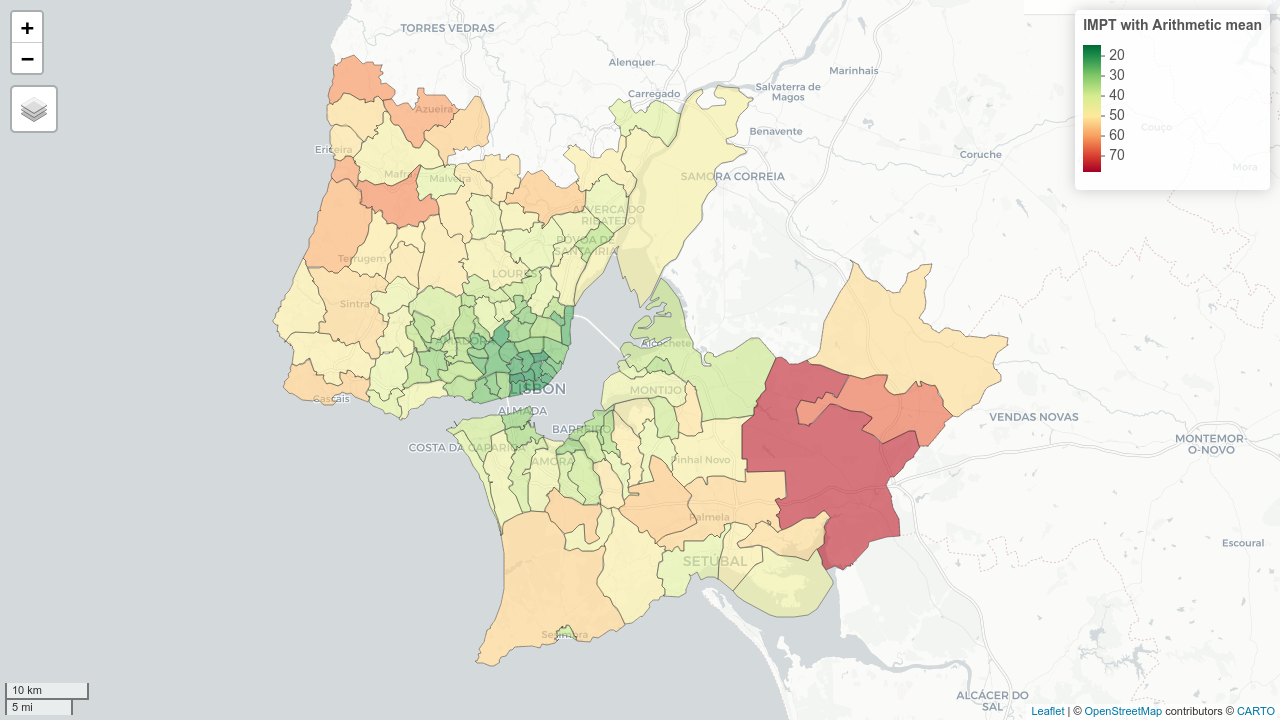
\includegraphics[keepaspectratio]{../documents/images/maps/impt_arithmetic.png}}

}

\subcaption{\label{fig-imt-arithmetic}Arithmetic mean}

\end{minipage}%
%
\begin{minipage}{0.33\linewidth}

\centering{

\pandocbounded{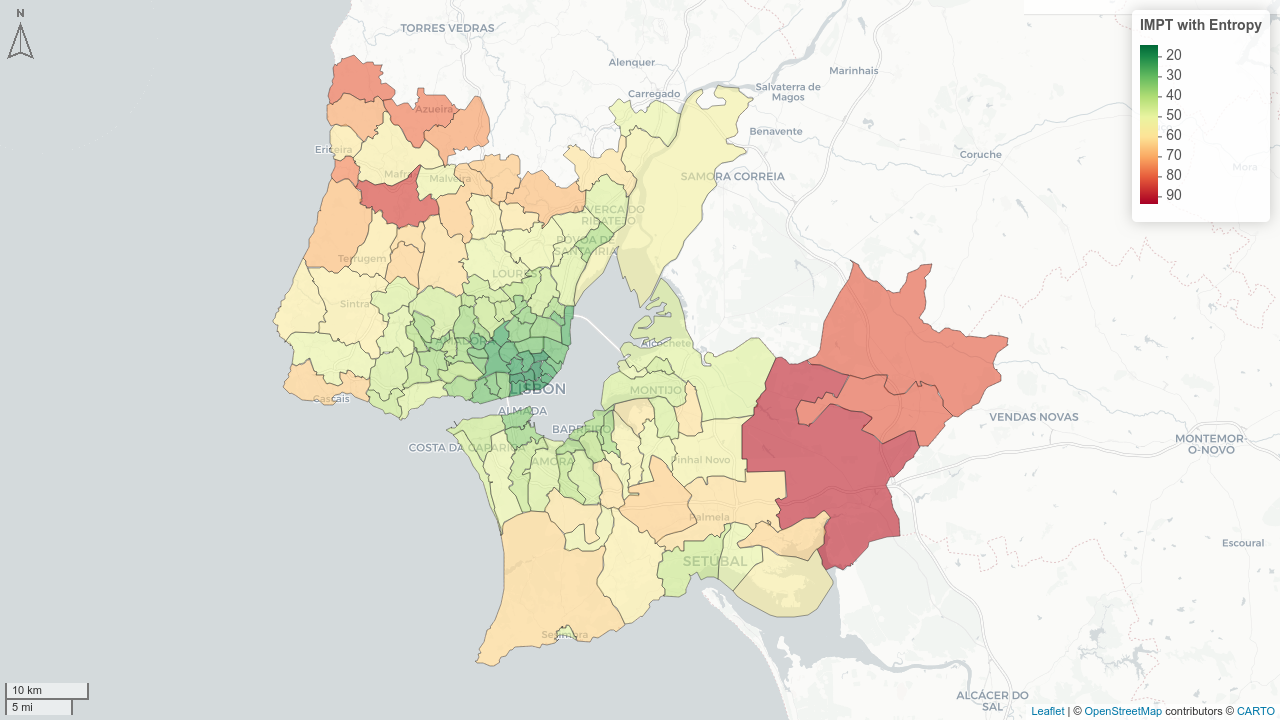
\includegraphics[keepaspectratio]{../documents/images/maps/impt_entropy.png}}

}

\subcaption{\label{fig-imt-entropy}Entropy-weighted mean}

\end{minipage}%

\caption{\label{fig-imt-methods}IMPT results for different aggregation
methods for all modes (with Navegante)}

\end{figure}%

\section{Results}\label{sec-results}

Figure~\ref{fig-meaningless} is generated using an R chunk.

\begin{figure}

\centering{

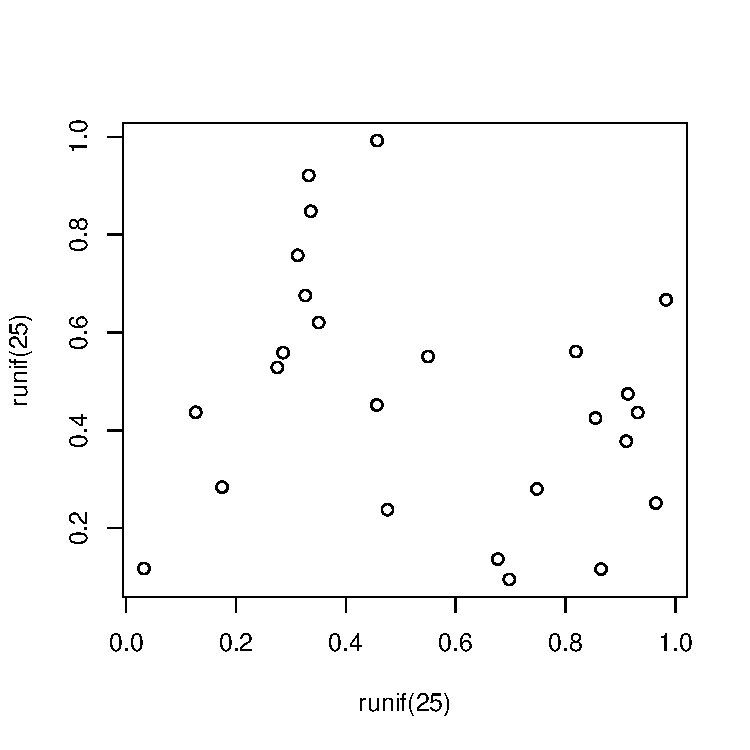
\includegraphics[width=0.5\linewidth,height=\textheight,keepaspectratio]{paper_files/figure-pdf/fig-meaningless-1.pdf}

}

\caption{\label{fig-meaningless}A meaningless scatterplot}

\end{figure}%

\section{Discussion}\label{sec-discussion}

\subsection{Limitations}\label{sec-limitations}

Tables can also be generated using R chunks, as shown in
Table~\ref{tbl-simple} example.

\begin{Shaded}
\begin{Highlighting}[]
\NormalTok{knitr}\SpecialCharTok{::}\FunctionTok{kable}\NormalTok{(}\FunctionTok{head}\NormalTok{(mtcars)[,}\DecValTok{1}\SpecialCharTok{:}\DecValTok{4}\NormalTok{])}
\end{Highlighting}
\end{Shaded}

\begin{verbatim}
Warning in attr(x, "align"): 'xfun::attr()' is deprecated.
Use 'xfun::attr2()' instead.
See help("Deprecated")
\end{verbatim}

\begin{verbatim}
Warning in attr(x, "format"): 'xfun::attr()' is deprecated.
Use 'xfun::attr2()' instead.
See help("Deprecated")
\end{verbatim}

\begin{longtable}[]{@{}lrrrr@{}}

\caption{\label{tbl-simple}Caption centered above table}

\tabularnewline

\toprule\noalign{}
& mpg & cyl & disp & hp \\
\midrule\noalign{}
\endhead
\bottomrule\noalign{}
\endlastfoot
Mazda RX4 & 21.0 & 6 & 160 & 110 \\
Mazda RX4 Wag & 21.0 & 6 & 160 & 110 \\
Datsun 710 & 22.8 & 4 & 108 & 93 \\
Hornet 4 Drive & 21.4 & 6 & 258 & 110 \\
Hornet Sportabout & 18.7 & 8 & 360 & 175 \\
Valiant & 18.1 & 6 & 225 & 105 \\

\end{longtable}

\section{Conclusions}\label{sec-conclusions}

This is the best paper ever.


\renewcommand\refname{References}
\bibliography{references.bib}



\end{document}
